\chapter[Regularizing Internal Solver Heuristics of Neural DEs]{Regularizing Internal Solver Heuristics of Neural Differential Equations}
\label{chapter:internal_solver_heuristics_regularized_neural_des}

How many hidden layers should you choose in your recurrent neural network? \citet{chen2018neural} showed that the answer could be found automatically by using a continuous reformulation, the neural ordinary differential equation, and allowing an adaptive ODE solver to effectively choose the number of steps to take. Since then the idea was generalized to other domains such as stochastic differential equations \citep{liu2019neural, rackauckas2020universal} but one fact remained: \textit{solving a neural differential equation is expensive, \& training a neural differential equation is even more so}.

In this thesis, we present a generally applicable method to force the neural differential equation training process to choose the least expensive option. We open the blackbox and show how using the numerical heuristics baked inside of these sophisticated differential equation solver codes allows for identifying the cheapest equations without requiring extra computation. However, ``opening the blackbox'' has several downsides -- they are \textit{harder to integrate into existing code-bases} and are \textit{more memory intensive}. Hence, we describe methods that exploit random sampling to leverage the benefits of ``opening the blackbox'' without actually requiring specialized training methods and the associated memory overhead.

The contents of this chapter has appeared previously in the following pre-prints / publications:
%
\begin{enumerate}
  \item \citep{pal2023locally} Pal, A., Edelman, A. and Rackauckas, C., 2023. Locally Regularized Neural Differential Equations: Some Black Boxes Were Meant to Remain Closed!. arXiv preprint arXiv:2303.02262.
  \item \citep{pal2021opening} Pal, A., Ma, Y., Shah, V. and Rackauckas, C.V., 2021, July. Opening the Blackbox: Accelerating Neural Differential Equations by Regularizing Internal Solver Heuristics. In International Conference on Machine Learning (pp. 8325-8335). PMLR.
\end{enumerate}
%

\section{Opening the Blackbox: Global Regularization using Local Error \& Stiffness Estimates}
\label{sec:global_regularization_using_local_error_and_stiffness_estimates}

\Cref{sec:adaptive_time_stepping} describes how larger local error estimates $\eest$ lead to reduced step sizes and thus a higher overall cost in the neural ODE training and predictions. Given this, we propose regularizing the neural ODE training process by the total local error in order to learn neural ODEs with as large step sizes as possible. Thus we define the regularizing term:
%
\begin{equation}
  \label{eq:reg_eest_global}
  \left(\mathcal{R}_{E}\right)_g = \sum_j \left(\eest\right)_j \cdot |\dt_j|
\end{equation}
%
summing over $j$ the time steps of the solution. This was done by accumulating the $\left(\eest\right)_j$ from the internals of the time stepping process at the end of each step. We note that this is similar to the regularization proposed in \citet{kelly2020learning}, namely:
%
\begin{equation}
  \label{eq:reg_global_kelly}
  \left(\mathcal{R}_{K}\right)_g = \int_{t_0}^{t_1} \left\|\frac{d^K z(t)}{dt^K}\right\| \dt
\end{equation}
%
where integrating over the $K^{th}$ derivatives is proportional to the principle (largest) truncation error term of the Runge-Kutta method~\citep{hairer1}. However, this formulation requires high order automatic differentiation (which then is layered with reverse-mode automatic differentiation) which can be an expensive computation~\citep{zhang2008computing} while \Cref{eq:reg_eest_global} requires no differentiation.

Similarly, the stiffness estimates (\Cref{sec:automatic_stiffness_detection}) at each step can be summed as:
%
\begin{equation}
  \label{eq:reg_stiffness_global}
  \left(\mathcal{R}_{S}\right)_g = \sum_j \left(\sest\right)_j \cdot |\dt_j|
\end{equation}
%
giving a computational heuristic for the total stiffness of the equation. Notably, both of these estimates $\left(\eest\right)_j$ and $\left(\sest\right)_j$ are already computed during the course of a standard explicit Runge-Kutta solution, making the forward pass calculation of the regularization term computationally free.


\section{Adjoints of Internal Solver Heuristics}
\label{sec:adjoints_of_internal_solver_heuristics}

Notice that $\left(\eest\right)_j = \sum_{i = 1}^s \left(b_i - \tilde{b_i}\right) \cdot k_i$ cannot be constructed directly from the $\func{z}{t_j}$ trajectory of the ODE's solution. More precisely, the $k_i$ terms are not defined by the continuous ODE but instead by the chosen steps of the solver method. Continuous adjoint methods for neural ODEs~\citep{chen2018neural, zhuang2021mali} only define derivatives in terms of the ODE quantities. This is required in order exploit properties such as allowing different steps in reverse and reversibility for reduced memory, and in constructing solvers requiring fewer NFEs~\citep{kidger2020hey}. Indeed, computing the adjoint of each stage variable $k_i$ can be done, but is known as discrete sensitivity analysis and is known to be equivalent to automatic differentiation of the solver~\citep{zhang2014fatode}. Thus to calculate the derivative of the solution simultaneously to the derivatives of the solver states, we used direct automatic differentiation of the differential equation solvers for performing the experiments~\citep{innes2018don}. We note that discrete adjoints are known to be more stable than continuous adjoints~\citep{zhang2014fatode} and in the context of neural ODEs have been shown to stabilize the training process leading to better fits \citep{gholami2019anode,onken2020discretize}. While more memory intensive than some forms of the continuous adjoint, we note that checkpointing methods can be used to reduce the peak memory \citep{dauvergne2006data}. We note that this is equivalent to backpropagation of a fixed time step discretization if the step sizes are chosen in advance, and verify in the example code that no additional overhead is introduced.


\section{Experimental Results for Global Regularization}
\label{sec:experimental_results_global_regularized_neural_des}


\section{Discussion on Global Regularization of Neural DEs}
\label{sec:discussion_on_global_regularization_of_neural_des}

Numerical analysis has had over a century of theoretical developments leading to efficient adaptive methods for solving many common nonlinear equations such as differential equations. Here we demonstrate that by using the knowledge embedded within the heuristics of these methods we can accelerate the training process of neural ODEs.

We note that on the larger sized PhysioNet and MNIST examples we saw significant speedups while on the smaller differential equation examples we saw only minor performance improvements. This showcases how the NFE becomes a better estimate of the total compute time as the cost of the ODE $f$ (and SDE $g$) increase when the model size increases.

This result motivates efforts in differentiable programming~\citep{wang2018backpropagation, abadi2019simple, rackauckas2020generalized} which enables direct differentiation of solvers since utilizing the solver's heuristics may be crucial in the development of advanced techniques. This idea could be straightforwardly extended not only to other forms of differential equations, but also to other ``implicit layer'' machine learning methods. For example, Deep Equilibrium Models (DEQ)~\citep{bai_deep_2019} model the system as the solution to an implicit function via a nonlinear solver like Bryoden or Newton's method. Heuristics like the ratio of the residuals have commonly been used as a convergence criterion and as a work estimate for the difficulty of solving a particular nonlinear equation~\citep{wanner1996solving}, and thus could similarly be used to regularize for learning DEQs whose forward passes are faster to solve. Similarly, optimization techniques such as BFGS~\citep{kelley1999iterative} contain internal estimates of the Hessian which can be used to regularize the stiffness of ``optimization as layers'' machine learning architectures like OptNet~\citep{amos2017optnet}. However, in these cases we note that continuous adjoint techniques have a significant computational advantage over discrete adjoint methods because the continuous adjoint method can be computed directly at the point of the solution while discrete adjoints would require differentiating through the iteration process. Thus while a similar regularization would exist in these contexts, in the case of differential equations the continuous and discrete adjoints share the same computational complexity which is not the case in methods which iterate to convergence. Further study of these applications would be required in order to ascertain the effectiveness in accelerating the training process, though by extrapolation one may guess that at least the forward pass would be accelerated.

\subsection{Limitations of Global Regularization using Error and Stiffness Estimates}
\label{subsec:limitations_of_using_error_and_stiffness_estimates}

While these experiments have demonstrated major performance improvements, it is pertinent to point out the limitations of the method. One major point to note is that this only applies to learning neural ODEs for maps $z(0) \mapsto z(1)$ as is used in machine learning applications of the architecture~\citep{chen2018neural}. Indeed, a neural ODE as an ``implicit layer'' for predictions in machine learning does not require identification of dynamical mechanisms. However, if the purpose is to learn the true governing dynamics a physical system from timeseries data, this form of regularization would bias the result, dampening higher frequency responses leading to an incorrect system identification. Approaches which embed neural networks into solvers could be used in such cases~\citep{shen2020deep,poli2020hypersolvers}. Indeed we note that such Hypereuler approaches could be combined with the ERNODE regularization on machine learning prediction problems, which could be a fruitful avenue of research. Lastly, we note that while either the local error and stiffness regularization was effective on each chosen equation, neither was effective on all equations and at this time there does not seem to be a clear a priori indicator as to which regularization is necessary for a given problem. While it seems the error regularization was more effective on the image classification tasks while the stiffness regularization was more effective on the time series task, we believe more experiments will be required in order to ascertain whether this is a common phenomena, possibly worthy of theoretical investigation.

\section{Randomized Local Regularization: Overcoming the shortcomings of Global Regularization}
\label{sec:randomized_local_regularization_overcoming_the_shortcomings_of_global_regularization}

\begin{table}[t]
  \centering
  \adjustbox{max width=\textwidth}{
    \centering
    \begin{tabular}{lcc}
      \toprule
      \thead{Sensitivity Algorithm} & \thead{Memory Requirement} & \thead{Memory Requirement with Local Reularization} \\
      \midrule
      Backsolve Adjoint \tocite & $\bigO{s}$ & $\bigO{s + \mathrm{stages}}$ \\
      Backsolve Adjoint with Checkpointing \tocite & $\bigO{s \times c}$ & $\bigO{s \times c  + \mathrm{stages}}$ \\
      Interpolating Adjoint \tocite & $\bigO{s \times t}$ & $\bigO{s \times t  + \mathrm{stages}}$\\
      Interpolating Adjoint with Checkpointing \tocite & $\bigO{s \times c}$ & $\bigO{s \times c + \mathrm{stages}}$ \\
      Quadrature Adjoint \tocite & $\bigO{\left(s + p\right) \times t}$ & $\bigO{\left(s + p\right) \times t + \mathrm{stages}}$ \\
      Direct Reverse Mode Differentiation & $\bigO{s \times t \times \mathrm{stages}}$ & $\bigO{\left(s \times t + 1\right) \times \mathrm{stages}}$ \\
      \bottomrule
    \end{tabular}
  }
  \caption{\textbf{Memory Requirements for various Sensitivity Algorithms for ODEs with Local Regularization}}
  \label{tab:memory_requirements_sensitivity_analysis_odes_with_local_reg}
\end{table}

In \Cref{subsec:limitations_of_using_error_and_stiffness_estimates}, we discussed the downsides of using global regularization with local error estimates. To summarize:
%
\begin{enumerate}
  \item Global Regularization relies on discrete sensitivity analysis, which is \textit{more memory intensive}.

  \item Global Regularization depends on AD tooling to support dynamic compute graphs in an efficient way, making it \textit{hard to incorporate into existing code-bases}.
\end{enumerate}
%
To get around these limitations, we developed a new technique using local sampling of error estimates at specific time points, rather than globally over the full interval. We deal with sampling the ``appropriate'' time point for regularization by two strategies:
%
\begin{itemize}
  \item \textbf{\Cref{alg:local_regularization_unbiased_sampling} Unbiased Sampling}: We random uniformly sample the time-point in the integration time span. Intuitively, since we will perform the training for ``a large number of steps,'' the learned dynamical system would end up being faster to solve ``everywhere'' over the time span.

  \item \textbf{\Cref{alg:local_regularization_biased_sampling} Biased Sampling}: Adaptive Time-Stepping Differential Equation Solvers naturally take more steps around the area, which is harder to integrate. We can bias the regularization to operate around parts of the dynamical system which are ``harder'' by sampling a time-point from the solution time points.
\end{itemize}
%

\begin{algorithm}[t]
  \caption{\textbf{Unbiased Sampling: Training}}
  \label{alg:local_regularization_unbiased_sampling}
  \begin{algorithmic}[1]
    \Function{$\texttt{ERNODE}_{\texttt{Unbiased}}$}{$x$, $f_\theta$, $t_{\texttt{span}}$}
    \State \texttt{Define} $\frac{du}{dt} = f_\theta(u, t)$
    \State $t_0, t_1 \gets t_{span}$
    \State $\treg \sim \mathbb{U}\left[t_0,~t_1\right]$
    \State $\texttt{sol} \gets \texttt{solve}(\frac{du}{dt}, \texttt{ DE Solver},~t_{\texttt{span}})$
    \State $u_{\treg} \gets \texttt{sol}(\treg)$
    \State Run single step for the solver with time-span $(\treg, t_1)$
    \State $\texttt{r} \gets $ Local Error Estimate $@ t=\treg$
    \State \Return{$\texttt{sol}, \texttt{r}$}
    \EndFunction
  \end{algorithmic}
\end{algorithm}

\subsection{Unbiased Sampling of Local Error Estimates}
\label{subsec:unbiased_sampling_of_local_error_estimates}

When training a Neural ODE, the integration time-span is fixed. Training any deep learning model involves several thousand steps. We compute the total local error estimate over the entire time-span when performing global regularization. For unbiased sampling, we hypothesize that if we regularize at random uniformly sampled time points in the time-span, the learned dynamical system will demonstrate similar properties in terms of NFE compared to global regularization. Our new regularization term becomes $\left(\mathcal{R}_{E}\right)_{\texttt{unbiased}}$ as:
%
\begin{gather}
  \left(\mathcal{R}_{E}\right)_{\texttt{unbiased}} = \left(\texttt{E}_{\texttt{Est}}\right)_{\treg} \cdot |\dt_{\treg}|\\
  \treg \sim \mathbb{U}[\texttt{tspan}]
\end{gather}
%

\begin{algorithm}[t]
  \caption{\textbf{Biased Sampling: Training}}
  \label{alg:local_regularization_biased_sampling}
  \begin{algorithmic}[1]
    \Function{$\texttt{ERNODE}_{\texttt{Biased}}$}{$x$, $f_\theta$, $t_{\texttt{span}}$}
    \State \texttt{Define} $\frac{du}{dt} = f_\theta(u, t)$
    \State $t_0, t_1 \gets t_{span}$
    \State $\texttt{sol} \gets \texttt{solve}(\frac{du}{dt}, \texttt{ DE Solver},~t_{\texttt{span}})$
    \State $\treg \sim \mathbb{U}\left(\texttt{sol}.t\right)$
    \State $u_{\treg} \gets \texttt{sol}(\treg)$
    \State Run single step for the solver with time-span $(\treg, t_1)$
    \State $\texttt{r} \gets $ Local Error Estimate $@ t=\treg$
    \State \Return{$\texttt{sol}, \texttt{r}$}
    \EndFunction
  \end{algorithmic}
\end{algorithm}

\subsection{Biased Sampling of Local Error Estimates}
\label{subsec:biased_sampling_of_local_error_estimates}

\begin{figure}[t]
  \centering
  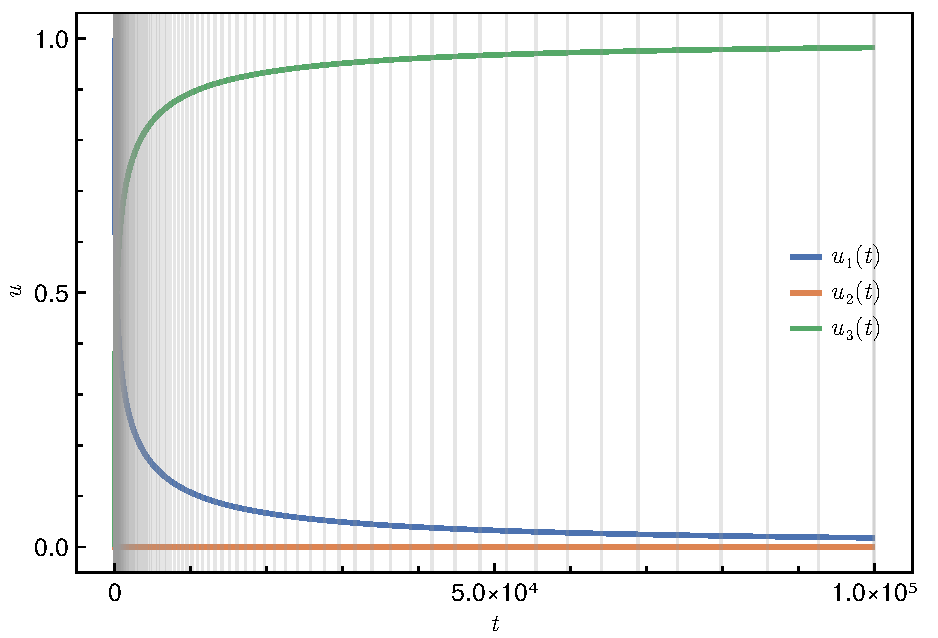
\includegraphics[width=0.5\linewidth]{../figures/regularizing_neural_des/biased_sampling_robertson_example}
  \caption{\textbf{Robertson Stiff ODE System}: Solving stiff systems like Robertson~\citep{robertson1966solution} (using Rodas5~\citep{piche1995stable}) involves spending around $75\%$ of the time in $t < 5000$ (i.e. $5\%$ of the time-span). The vertical lines denote the time-points at which the ODE System was solved.}
  \label{fig:robertson_stiff_system}
  \vspace{-1.5em}
\end{figure}


Consider a simple scenario where the learned dynamics of the DE is harder to solve in $\left[0.25, 0.35\right]$, and we are solving the DE from $t_0 = 0$ to $t_1 = 1$. Our primary aim is to modify the learned system s.t. it becomes simpler to solve in $\left[0.25, 0.35\right]$. If we use unbiased sampling, the probability that we regularize at $\treg \in \left[0.25, 0.35\right]$ is $0.1$ (which is low). The problem gets even more severe if the range is lowered. An extreme version of this problem is observed for stiff systems like Robertson's Equations~(See \Cref{fig:robertson_stiff_system}) where $75\%$ of the time is spent in solving $5\%$ of the problem. We note that these extreme scenarios rarely occur for traditional deep learning tasks since \citet{pal2021opening} observed minor speedups using stiffness regularization. However, the problem that some parts of the dynamical system are harder to integrate persists, and designing a regularization scheme targeting those parts is highly desirable.

We considered a simple scenario where the learned dynamical system was fixed. However, while training NDEs, this system evolves with training, and apriori predicting the more difficult portions to integrate is not feasible. Adaptive solvers take more frequent steps in the parts of the DE where it is harder to integrate. \citet{anantharaman2020accelerating} leveraged this property of adaptive solvers to learn surrogates for stiff systems. Since these solvers adapt to concentrate around the most numerically difficult time points, we automatically obtain the time points where we want to regularize the model. Hence, for our biased sampling regularize, we uniformly sample the regularization timepoint $\treg$ from the time points at which the solver solved the differential equation.

\section{Adjoint for Local Regularized Neural Differential Equations}
\label{sec:adjoint_for_local_regularized_neural_differential_equations}

\section{Experimental Results for Local Regularization}
\label{sec:experimental_results_local_regularized_neural_des}

\section{Discussion on Local Regularization of Neural DEs}
\label{sec:discussion_on_local_regularization_of_neural_des}

\section{Conclusion}
\label{sec:conclusion}
